\begin{figure}[h]
    \centering    
{\footnotesize
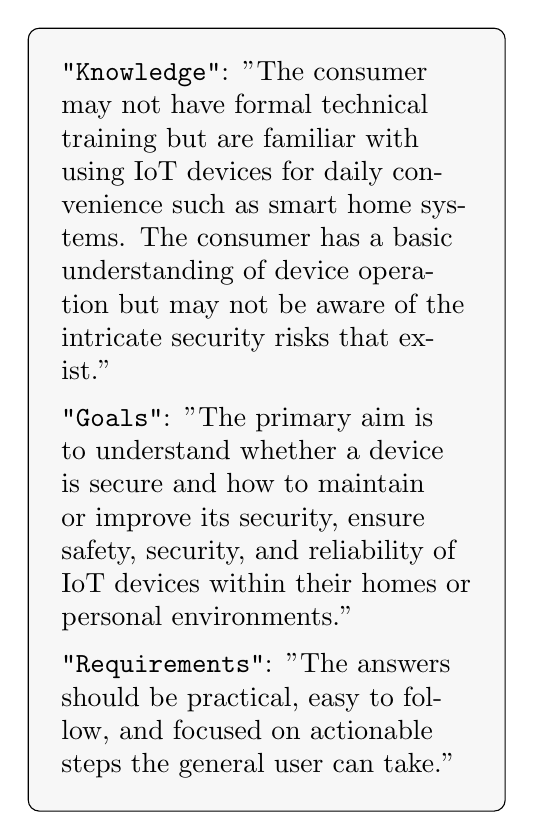
\begin{tikzpicture}
% Draw rounded rectangle with shadow
\node[rectangle, rounded corners, draw=black, fill=black!3!white, text width=0.43\textwidth, inner sep=12pt, align=left] (box) {
\textbf{\texttt{"Knowledge"}}: "The consumer may not have formal technical training but are familiar with using IoT devices for daily convenience such as smart home systems. The consumer has a basic understanding of device operation but may not be aware of the intricate security risks that exist."
\vspace{5pt}\\
\textbf{\texttt{"Goals"}}: "The primary aim is to understand whether a device is secure and how to maintain or improve its security, ensure safety, security, and reliability
of IoT devices within their homes or personal environments."
\vspace{5pt}\\
\textbf{\texttt{"Requirements"}}: "The answers should be practical, easy to follow, and focused on actionable steps the general user can take."
};
\end{tikzpicture}
}
\caption{The background for consumer utilized to guide the \chatiot\ to generate consumer-friendly outputs.}
\label{fig:usecasedef-consumer}
\end{figure}